% fig-three-layer — §3, the three-layer enforcement architecture.
% Standalone-buildable AND \input-able. Monochrome, sober. Reusable.
\documentclass[border=4pt]{standalone}
\usepackage{tikz}
\usetikzlibrary{positioning}
\begin{document}
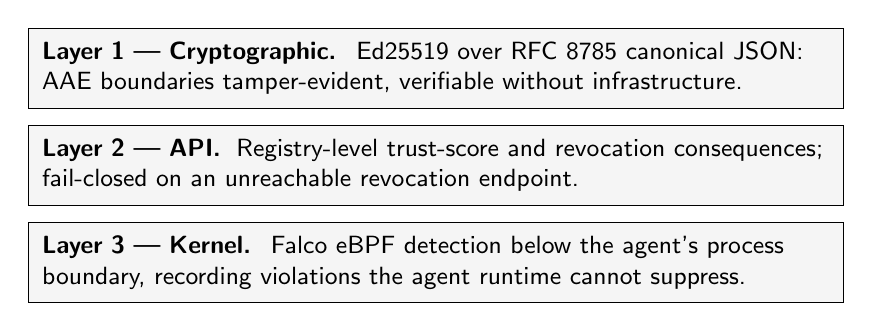
\begin{tikzpicture}[
  lyr/.style={draw=black, thin, align=left, font=\small\sffamily, fill=black!4,
              text width=100mm, inner sep=5pt},
  node distance=2mm
]
\node[lyr] (l1) {\textbf{Layer 1 — Cryptographic.}\; Ed25519 over RFC~8785 canonical JSON: AAE boundaries tamper-evident, verifiable without infrastructure.};
\node[lyr, below=of l1] (l2) {\textbf{Layer 2 — API.}\; Registry-level trust-score and revocation consequences; fail-closed on an unreachable revocation endpoint.};
\node[lyr, below=of l2] (l3) {\textbf{Layer 3 — Kernel.}\; Falco eBPF detection below the agent's process boundary, recording violations the agent runtime cannot suppress.};
\end{tikzpicture}
\end{document}
